\section{Задача 1.35}
\subsection{Задание:}
Вычислить $ \det A, A = \{ a_{ij} \} |, i = \overline{1,n}, j = \overline{1,n}, a_{ij} = \min (i,j) $
\subsection{Решение:}
Докажем методом мат. индукции что $ \det A = 1 $:
\\
Проверим базу индукции: $ |1| = 1 $
\\
Допустим что утверждение верно для $ n $, тогда докажем что оно будет верно для $ n + 1 $:
\\[1em]
$
	\begin{vmatrix}
		     1 &      1 & \cdots &      1 &       1 \\
		\vdots & \vdots & \ddots & \vdots &  \vdots \\
		     1 &      2 & \cdots &      n &       n \\
		     1 &      2 & \cdots &      n &   n + 1 \\
	\end{vmatrix}_{n + 1}
	=
	\begin{vmatrix}
		     1 &      1 & \cdots &      1 &       1 \\
		\vdots & \vdots & \ddots & \vdots &  \vdots \\
		     1 &      2 & \cdots &      n &       n \\
		     0 &      0 & \cdots &      0 &       1 \\
	\end{vmatrix}_{n + 1}
	=
	\begin{vmatrix}
		     1 &      1 & \cdots &      1  \\
		\vdots & \vdots & \ddots & \vdots  \\
		     1 &      2 & \cdots &      n  \\
	\end{vmatrix}_n
$
\\[1em]
В силу мат. индукции предположение доказано.
\subsection{Компьютерная проверка в среде Wolfram Mathematica:}
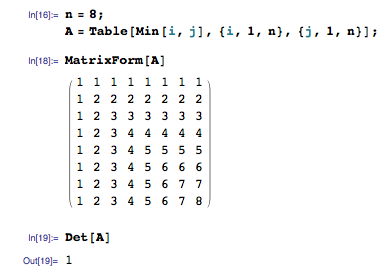
\includegraphics[scale=0.6]{task/1_35/screen1.png}
\subsection{Вывод:}
Компьютерная проверка показала что утверждение верно.
